\documentclass[11pt, a4paper]{article}
\usepackage[ngerman]{babel}
\usepackage{color}
\usepackage{graphicx}
\graphicspath{{./images/}}
\usepackage{hyperref}
% \usepackage{geometry}
% \geometry{
% 	a4paper,
% 	total = {150mm, 247mm},
% 	left= 40mm,
% 	right = 20mm,
%	bottom = 250mm,
%	top = 250mm,
% }


\usepackage{listings}
\usepackage{color}

\definecolor{codegreen}{rgb}{0,0.6,0}
\definecolor{codegray}{rgb}{0.5,0.5,0.5}
\definecolor{codepurple}{rgb}{0.58,0,0.82}
\definecolor{backcolour}{rgb}{0.95,0.95,0.92}

\lstdefinestyle{mystyle}{
    backgroundcolor=\color{backcolour},   
    commentstyle=\color{codegreen},
    keywordstyle=\color{magenta},
    numberstyle=\tiny\color{codegray},
    stringstyle=\color{codepurple},
    basicstyle=\ttfamily\footnotesize,
    breakatwhitespace=false,         
    breaklines=true,                 
    captionpos=b,                    
    keepspaces=true,                 
    numbers=left,                    
    numbersep=5pt,                  
    showspaces=false,                
    showstringspaces=false,
    showtabs=false,                  
    tabsize=2
}
\lstset{style=mystyle}


\newif\ifproofread

\newcommand{\changemarker}[1]{%
\ifproofread
\textcolor{red}{#1}%
\else
#1%
\fi
}



\hypersetup{
    colorlinks=true,
    linkcolor=blue,
    filecolor=magenta,      
    urlcolor=cyan,
    pdftitle={Overleaf Example},
    pdfpagemode=FullScreen,
    }

\begin{document}
\section{Notes}

Latex, Mathematica, MS Word etc.

\bigskip

\noindent German or English

\bigskip

\noindent Plan of a Project(6p. min)

\bigskip

\begin{enumerate}
	\item Introduction(1p.)\\
		state-of-the-art, general knowledge, popular summary
	\item Problem formulation(1p.)\\
		specific task, as a part of a general picture, challanges
	\item Mainpart: Approches and new results(2-3p.)\\
		seperate Mathematica code[i.a. for presentation]\\
		graphs, tables, videos, easy-to-use, appeling and interactive
	\item Conclusion(1p.)\\
		summary of the main results, gained knowledge, hurdles, broader interest
	\item Bibliography
\end{enumerate}

\newpage

\tableofcontents

\newpage

\section{Einführung}

Das Lösen eines Labyrinths mit Hilfe komplexer Algorithmen, welche von \\höheren Lebensformen angewandt werden können, ist eine Aufgabe in der es inzwischen darum geht Algorithmen zu finden, welche immer schneller und weniger Speicher aufwendig sind. 

\bigskip

Mit Blick auf niedrigere Lebewesen wie Käfer, Milben und ähnliches kommt die Frage auf ob es möglich ist ein Labyrinth auch mit simplen Algorithmen oder ganz ohne Algorithmen diese zu lösen. In dem wissenschaftlichen Artikel "Development of an automatic truntable-type multiple T-maze device and observation of pill bug behavior" wird das Bewegungsverhalten von Rollasseln (Armadillidiidae) in einem unendlichen Labyrinth untersucht, um festzustellen, ob einer Wiederholung von Richtungswechseln in die gleiche Richtung eine Fehlfunktion ist. Es wird von einer Fehlfunktion gesprochen, da bei Organismen mit simplen Nervensystemen davon ausgegangen wird, dass diese Entscheidungen mechanisch getroffen werden. In der Studie zeigt aber, dass eine wiederholte Drehung in eine Richtung in Maßen angewandt wird um einen Bewegungsablauf aus zu führen.

\bigskip

Um Labyrinthe zu lösen werden Algorithmen bewusst oder unbewusst angewandt. So werden für Computeralgorithmen Labyrinthe in Graphen umgewandelt, wobei jede Kreuzung im Labyrinth zu einem Knoten im \\ Graphen wird und die Strecke zwischen diesen Kreuzungen zu Kanten im Labyrinth. Um nun den das Labyrinth zu lösen muss lediglich die Kombination von Knoten und Kanten gefunden werden welche zwischen dem Start und dem Ziel des Labyrinths liegen. Auf dieser Grundlage kann man die verschiedensten Suchalgorithmen aus der Graphentheorie anwenden um die Verbindung zwischen den zwei Knoten zu finden. Um in einem Labyrinth mit mehreren Lösungswegen den besseren zu finden, ist es möglich die Kanten zu gewichten, ihnen Werte basierend auf bestimmten Eigenschaften zuzuweisen, wie zum Beispiel die Länge des Weges oder die Schwierigkeit diesen zu passieren.

\bigskip

\proofreadtrue

\changemarker{Popluare summary} \\
\href{https://www.jus.uio.no/english/research/phd/thesis-evaluation/evaluation/popular-science-summary.html}{How To write Popular summary}
\proofreadfalse

\newpage

\section{Problem}

Die folgenden Seiten befassen sich mit Problem ein Labyrinth zu lösen. Dabei soll ein Käfer dieses Labyrinth durchlaufen, während dieses Durchlaufs werden die Anzahl der Schritte sowie die Zeit die der Käfer benötigt gemessen. Ein Schritt findet statt, wenn der Käfer eine Position im Labyrinth weitergeht. Eine Zeiteinheit verstreicht, wenn der Käfer eine Aktion \\ durchführt, wobei eine Aktion ein Schritt sein kann oder das Prüfen ob ein Schritt möglich ist. Dieser Versuch wird in zwei Variationen durchgeführt, in der ersten Variation ist es dem Käfer möglich in alle vier Himmelsrichtung zu laufen. In der zweiten Variation kann der Käfer aber nicht rückwärts gehen und muss sich somit drehen, dies erhöht die Zeit ebenfalls.

\bigskip

In diesem Experiment gilt es, herauszufinden wie sich die Größe des Labyrinths auf die Zeit und die Schritte, welche der Käfer benötigt auswirken. Genauer wird geguckt in welchem Verhältnis Schritte und Zeit in einem einzelnen Durchlauf stehen und in welchem Verhältnis sie in Durchläufen mit unterschiedlich großen Labyrinthen stehen. Darauf hin gilt es die Ergebnisse der ersten Variante mit denen der zweiten Variante zu vergleichen. Um das Experiment erfolgreich durchführen zu können, gilt es sicherzustellen, dass das Labyrinth auch lösbar ist, also ein Weg zwischen Start und Ziel immer besteht. Aber nicht nur das Labyrinth muss an sich lösbar sein, auch der Käfer muss mit einer simplen Bewegungsabfolge durch das Labyrinth kommen ohne sich an einer Stelle im Kreis zu drehen oder sich gar nicht mehr zu bewegen. Dem ist hinzuzufügen, dass im nicht Kreisdrehen heißt das er irgendwann aus diesem Kreis wieder heraus kommt, nicht das er nicht öfters die gleiche Strecke ablaufen darf.

\bigskip

\proofreadtrue

\changemarker{as a part of a general picture}

\proofreadfalse

\newpage

\section{Aufbau}

\subsection{Erzeugen des Labyrinths}

Um dem Käfer die Möglichkeit zu geben das Labyrinth in jedem Fall lösen zu können, muss dieses ein "perfektes" Labyrinth sein. Das heißt, dass es möglich ist von jedem Punkt im Labyrinth zu jedem anderen zu kommen. Zudem hat dieses Labyrinth weder Schleifen noch Pfade die sich kreuzen. Weiter hin sollen die Labyrinthe zufällig erzeugt werden, um den Ablauf des Programms zu vereinfachen und so wenig wie mögliche Durchläufe auf dem gleichen Labyrinth zu haben.

\bigskip

Ein Labyrinth ist wie in 2. erklärt zu verstehen. Um ein perfektes Labyrinth aus einem Graphen zu erzeugen, muss man einen Spannbaum aus diesem Graphen finden. Um dies zu tun gibt es 11 verschiedene Algorithmen. Des weiteren wird sich mit dem Kruskal Algorithmus befasst. 

\bigskip

Der Kurskal Algorithmus findet in einem gewichteten Graphen den minimalen Spannbaum, in dem er die minimale Summe aller Gewichte findet und die Konten so verbindet. Dabei fängt er mit dem niedrigsten Gewicht an und verbindet die zwei Konten zu einem Baum. Dieser Schritt wird nun wiederholt, bis alle Konten mit einander verbunden sind. Sollte währenddessen ein Konten mit einem Baum oder ein Baum mit einem Baum verbunden werden, so werden diese zu einem einzigen Baum zusammen gefasst. Dabei ist aber zu beachten, dass nur Konten mit einander verbunden werden, wenn diese nicht im gleichen Baum sind. Da sonst eine Schleife entstehen würde. Dadurch entsteht am Ende ein minimaler Spannbaum auf dem Graphen.  

\bigskip

Um ein Labyrinth zu erstellen sind die Gewichte der Kanten nicht weiter relevant, wodurch man sie weg lassen kann. Das führt dazu, dass die Knoten nicht anhand der Gewichte verbunden werden, sonder zufällig zwei Kontenpaare ausgewählt werden und anschließend verbunden. Es entsteht ein zufälliger Kruskal Algorithmus.
Die Umsetzung erfolgt wie folgt.


Es wird die Höhe und Breite des Labyrinths verdoppelt um die Wände einzufügen und eins addiert um das Labyrinth auf allen Seiten mit Wänden zu umfassen. Folgend werden nochmal zwei addiert um die Aussenwände "zwei dick" zu machen.(Dies wird später erklärt.)
\begin{lstlisting}[language = Python]
# Bug.py
def __init__(self, h, w):
        self.H = 2*h+3
        self.W = 2*w+3
        self.grid = None
\end{lstlisting}

Anschließend wird ein Gitter aus Einsen erstellt und in der dritten Zeile und Spalte die Eins auf Null gesetzt um einen Knoten zu symbolisieren. Dies wird mit einer Lücke von Eins nach rechts und unten fortgesetzt und einer Liste an Konten hinzugefügt. Anschließend werden alle verbleibenden Einsen als Kanten einer Liste hinzugefügt. Zu letzt werden die Kanten gemischt.

\begin{lstlisting}[language = Python]
# Bug.py
def generate(self):
        self.grid = np.empty((self.H,self.W), dtype=np.int8)
        self.grid.fill(1)
        
        forest = []
        for row in range(2,self.H-2, 2):
            for col in range(2,self.W-2, 2):
                forest.append([(row,col)])
                self.grid[row][col] = 0
        
        edges = []
        for row in range(3, self.H-2, 2):
            for col in range (2,self.W-2, 2):
                edges.append((row,col))
        for row in range(2, self.H-2, 2):
            for col in range (3,self.W-2, 2):
                edges.append((row,col))
        
        shuffle(edges)
\end{lstlisting}

Aus der Liste der Kanten wird solange das erste Element heraus genommen, bis die Länge der Knoten Eins beträgt. Das herausgenommenen Element wird geprüft ob es Konten über und unter sich oder links und rechts von sich hat. Anschließend wird die Position der Knoten in der Liste der Konten aufaddiert und in tree1 und tree2 gespeichert.

\begin{lstlisting}[language = Python]
# Bug.py
while len(forest) > 1:
            ce_row, ce_col = edges[0]
            edges = edges[1:]
        
            tree1 = 0
            tree2 = 0
        
            if ce_row % 2 == 1:
                for i,j in enumerate(forest):
                    if(ce_row - 1, ce_col) in j:
                        tree1 += i
                    else:
                        tree1 += 0
                for i,j in enumerate(forest):
                            if(ce_row + 1, ce_col) in j:
                                tree2 += i
                            else:
                                tree2 += 0
                
            else:
                for i,j in enumerate(forest):
                    if(ce_row, ce_col - 1) in j:
                        tree1 += i
                    else:
                        tree1 += 0
                for i,j in enumerate(forest):
                            if(ce_row, ce_col + 1) in j:
                                tree2 += i
                            else:
                                tree2 += 0
\end{lstlisting}

Wenn diese Positionen nicht gleich sind, heißt wenn sie sich nicht im gleichen Baum befinden, werden sie verbunden und zu einem Baum zusammen gefügt. Wenn nur noch ein Baum in der Liste ist bricht die while-Scheife ab und der minimale Spannbaum wurde gefunden.

\begin{lstlisting}[language = Python]
if tree1 != tree2:
                new_tree = forest[tree1] + forest[tree2]
                temp1 = list(forest[tree1])
                temp2 = list(forest[tree2])
                forest = [
                        x for x in forest if x != temp1
                        ]
                forest = [x for x in forest if x != temp2]
                forest.append(new_tree)
                self.grid[ce_row][ce_col] = 0
\end{lstlisting}

\subsection{Durchlaufen des Labyrinths}

Nach dem das Labyrinth erzeugt wurde liegt eine Liste von Listen mit Nullen und Einsen gefüllt vor, wobei eine Eins eine Wand symbolisiert und eine Null einen Weg. 

\bigskip

Um nun das Labyrinth durchlaufen zu können, wird als Startpunkt die obere linke Ecke gewählt und als Ziel die untere rechte Ecke.Des weiteren gilt es zu beachten, dass eine Bewegung immer um zwei Felder passiert, da die Wände ebenfalls als Feld gewertet werden. Wir also bei einem 3x3 Feld bis zu fünf Schritten in eine Richtung laufen könnten, statt 3.

\bigskip

Im ersten Versuch einen simplen Bewegungsablauf zu finden bestand der Versuch daraus, im Uhrzeigersinn von oben beginnend zu prüfen ob sich in die Richtung eine Wand befindet. Ist dies der Fall wird die nächste Richtung geprüft, ansonsten bewegt sich der Käfer ein Feld in diese Richung. 

Bei diesem Versuch trat jedoch das Problem auf das der Käfer das Labyrinth nicht lösen kann, da er sobald er nach unten geht im nächsten schritt zwindend wieder nach oben geht. Somit bewegt sich der Käfer effektiv auf zwei Feldern. Und konnt mehrere Felder nur nach oben oder links laufen. Aufgrund seiner Startposition war die Bewegung nach oben jedoch nicht möglich.

\bigskip

Im zweiten Versuch wurde nur die Reihenfolge der Richtungen in welcher geprüft wird geandert. Es ging immer noch im Uhrzeigersinn, jedoch wurde nun zuerst die rechte Seite geprüft.

Das Problem, im zweiten Versuch bewegte sich der Käfer nun nach links und rechts zwischen den selben zwei Feldern bewegte. 

\bigskip

Diese beiden Versuche ergaben das egal von welcher Richtung im Uhrzei-gersinn oder dagen gegangnen würde, nach wenigen Schritten würde der Käfer also nur noch zwischen zwei Punkten springen. Somit konnten zwar mit Glück kleinere Labyrinthe gelöst werden aber dies geschar nicht zuverlässig und war somit nicht nutzbar oder auf größere Labyrinthe anwendbar.

\bigskip

Der dritte Versuch basiert auch auf dem Prüfen der Richtung im Uhrzei-gersinn, nur das in diesem die Ausgangsrichtung zufällig gewählt wird. Dazu wird eine Zahl zufällig mit der in Python verbauten random Bibliothek erzeugt welches als ihren Kern den Mersenne Twister Generator verwendet. Dies zufällige Zahl zwischen 0 und 3 entspricht jeweils einer Richtung, wobei 0 für rechts steht und von dort aus im Uhrzeigersinn gegangen wird. In dem Versuch wo der Käfer nicht rückwärts laufen kann, wird, wenn er rückwärts laufen muss, der Käfer einmal rotiert, anschließend prüft er nach vorne und bewegt sich dann zur Seite. Auf diese Weise liessen sich alle Labyrinthgrößen lösen mit denen getestet wurde. Diese Tests liefen bis zur größe 20.

\subsection{Daten sammeln und speichern}

Gespeichert wird welcher Durchlauf es insgesamt war, wie groß das Labyrinth war, welcher Durchlauf es für die bestimmte größe war, in welcher Zeit und mit wie vielen Schritten der Durchlauf abgeschlossen wurde und wie das Labyrinth aussah. Die Zeit wird berechnet jenachdem ob eine Prüfung nach einer Wand statgefunden hat oder ob ein Schritt gemacht wurde, heißt wenn ein Schritt gemacht wird, wird die Prüfung nach einer Wand nicht auf die Zeit gerechnet. Dies ist so vorzustellen als würde der Käfer gegen die Wand rennen, wenn eine dort ist hat er eine Zeiteinheit oben drauf wenn keine dort ist hat er sie ebenfalls oben drauf ist aber einen Schritt weiter. Die Schritter werden nur berechnet, wenn sich der Käfer ein Feld weiter bewegt hat.
Diese Daten werden anschließend für jeden Labyrinthgröße in einer CSV-Datei gespeichert.

\section{Auswertung}

Es wurden Labyrinthe von der Größe drei bis zur Größe 38 für den Versuch verwendet. Jedes Labyrinth wurde dabei 100 mal gelöst und die Daten gespeichert und für diese Auswertung herangezogen. 

\bigskip

Bei der Betrachtung der Lösung eines einzelen Labyrinths fällt auf, dass die Zeit und Schritte, welche benötigt wurden um dieses Labyrinth zu lösen, bis auf ein paar Ausreißer, in einem gewissen Bereich gleich nah aneinander liegen. Ein hervorragendes Beispiel dafür ist der Druchlauf 29, zu sehen in Abbildung \ref{fig:Plot 29}, aus dem ersten Versuch. Dort ist nur ein Ausreißer deutlich zu erkenne, ansonsten liegen die Werte nah bei einander.

\begin{figure}[h]
\centering
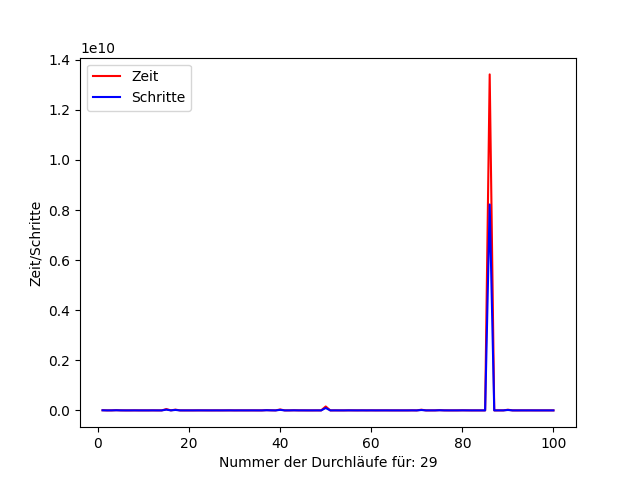
\includegraphics[scale=.5]{29.png}
\caption{Plot Durchlauf 29, erster Versuch}
\label{fig:Plot 29}
\end{figure}

Zu beachten ist jedoch, dass die Werte nicht durchgehend die selben sind, abgesehen von den zuvor erwähnten Ausreißern, wie man es aus Abbildung \ref{fig:Plot 29} annehmen kann. Dass die Werte unterschiedlich sind und doch in der Nähe der anderen Werte liegen sieht man in Abbildung \ref{fig:Plot 3}, wo der Durchlauf 3 des ersten Versuches zu sehen ist.


\begin{figure}[h]
\centering
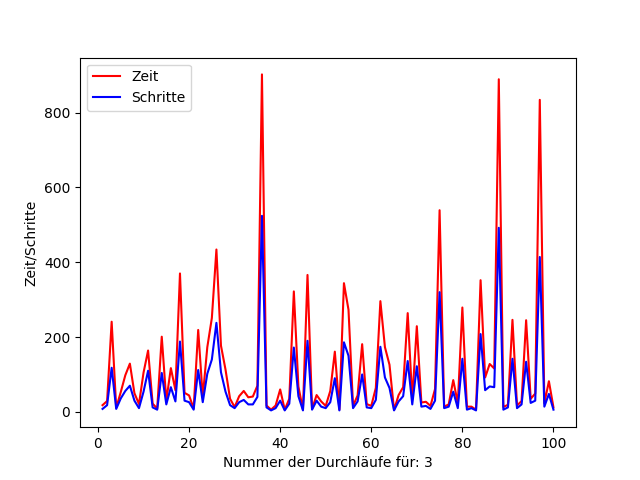
\includegraphics[scale=.5]{3.png}
\caption{Plot Durchlauf 3, erster Versuch}
\label{fig:Plot 3}
\end{figure}

Nimmt man nun den Durchschnitt der Zeit und Schritte jeder Labyrinthsgröße und ermittelt dafür jeweils den Durchschnitt, so kann man anhand eines Plots ablesen, wie sich die benötigten Schritte und Zeit im Verhältnis zur Labyrinthsgröße verhalten.  
In Abbildung \ref{fig:Plot v1} ist der erste Versuch abgebildet. In diesem ist zu erkennen, dass sich bis Labyrinthgröße 22 keine starke Veränderung der benötigten Zeit oder Schritte einstellt. Bei Labyrinthgröße 23 ist der erste kleine Ausschlag zu erkennen und bei Labyrinthgröße 29 und 31 befinden sich die ersten beiden starken Ausschläge, wobei sich Größe 30 wieder in der Nähe der Größen bis 22 befindet. Anschließend findet ein leichter anstieg statt und ein starker Ausschlag bei Größe 36. 
Wird nun eine Regressionskurve eingefügt, so ist zu erkennen, dass der Anstieg einer Exponentialfunktion ähnelt.

\begin{figure}[h]
\centering
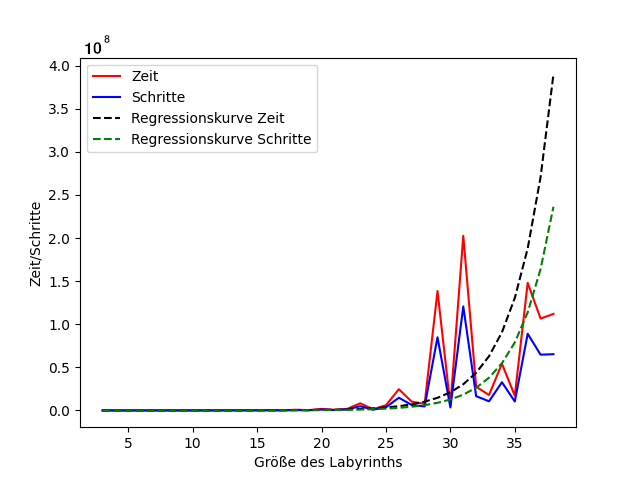
\includegraphics[scale=.5]{v1Aus.png}
\caption{erster Versuch}
\label{fig:Plot v1}
\end{figure}




\end{document}
